\section{Research Design}
\label{sec:design}

\subsection{Type of study}

This is an \emph{experimental, comparative classification study}. It is experimental because the quantity of interest is the effect of a controlled intervention, the composition of the training data, on a measured outcome, with everything else held fixed. It is comparative because the proposed method is judged against baselines and ablations trained under the same budget. It is a classification study because the model's output is a decision, per relation, about whether that relation holds for the queried primitives. Fig.~\ref{fig:design} shows the design.

\begin{figure}[tbp]
  \centering
  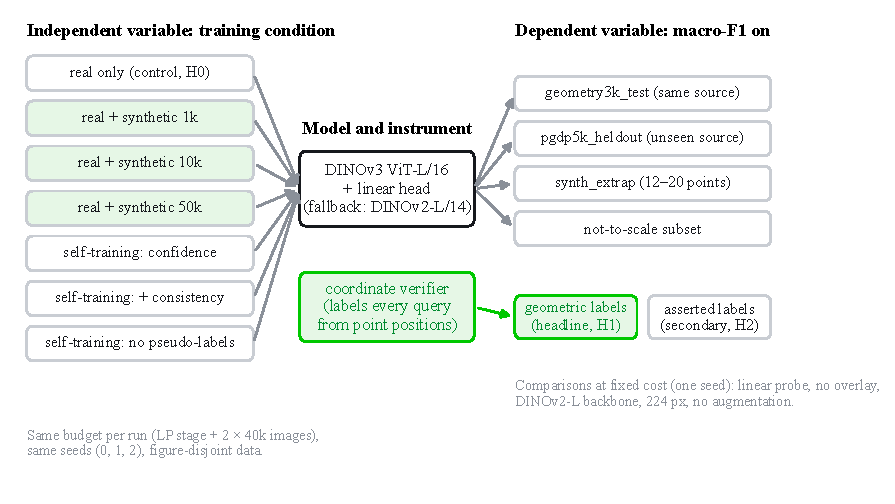
\includegraphics[width=\textwidth]{fig_design}
  \caption{Research design. Training conditions (left) vary the data; the model and the verifier are fixed; the outcome is macro-F1 on four evaluation sets against two label sets. Cheaper one-seed comparisons (bottom right) isolate design choices.}
  \label{fig:design}
\end{figure}

\subsection{Unit of analysis, inputs and outputs}

The unit of analysis is a \emph{query}: one diagram together with one tuple of its primitives. Segment pairs are queried for \rel{parallel}, \rel{perpendicular} and \rel{equal\_length}; point--circle pairs for \rel{on\_circle}; segment--circle pairs for \rel{tangent}; and point--segment triples for \rel{collinear}. The input to the model is the diagram image with the queried primitives highlighted (Section~\ref{sec:preprocessing}). The output is a six-dimensional vector of probabilities, one per relation, with an \emph{applicability mask} that excludes the relations a query kind cannot have: a segment pair can be both perpendicular and equal in length, but it cannot lie on a circle. A query with no positive relation is the \rel{none} case; it is represented as the all-zero vector rather than as a seventh class, so that multi-label queries remain expressible.

Primitive detection is out of scope by design: points, segments and circles come from the dataset annotations (Section~\ref{sec:dataset}). This isolates relation perception, the object of the hypotheses, from object detection, which the diagram-parsing literature already covers \cite{zhang2022pgdp}.

\subsection{Variables}

\paragraph{Independent variable.} The training condition. The primary contrast is \emph{real data only} against \emph{real data plus verifier-labelled synthetic diagrams}, at synthetic set sizes of \scalingSizes{} diagrams, every run at the same number of training images. A second contrast, within the self-training extension, is the pseudo-label filter: confidence alone, confidence with a deductive-consistency check, and a control that continues training without pseudo-labels.

\paragraph{Dependent variable.} Macro-F1 over the six relations, measured against the \emph{geometric} labels produced by the verifier, on four evaluation sets: the in-distribution test split, a held-out source never seen in training, a synthetic extrapolation set whose diagrams have \synthExtrapPointsMin--\synthExtrapPointsMax{} points (more than any training diagram), and the subset of real test diagrams flagged as not drawn to scale. The same predictions are also scored against the \emph{asserted} (human) labels; this second score is the outcome for \Htwo.

\paragraph{Controlled variables.} The backbone, resolution, augmentation, optimiser, schedule, training budget, random seeds, query enumeration and evaluation protocol are identical across the conditions of a contrast. Each design choice that could itself matter (backbone family, input resolution, augmentation, the highlight overlay) is varied once in a separate single-seed comparison (Section~\ref{sec:baselines}) rather than confounded with the main contrast.

\subsection{Why this design fits the hypotheses}

\Hone{} is a claim about a difference between two training conditions on two particular evaluation sets, so it needs a controlled contrast at equal budget, several seeds to estimate run-to-run variation, and evaluation sets that are provably disjoint from training (by figure, not by problem). \Hzero{} is the complement of \Hone{} under that same variation. \Htwo{} is a claim about two label sets on the same predictions, so every test query must carry both labels, which the two-label design provides. A purely predictive or applied design, which would optimise one model on one benchmark, could not separate the effect of the data from the effect of the labels; the comparative design does.
